
\section{Summary and outlook}
\label{sec:summary}

A tensor network formulation for lattice fermions has been constructed, based on the introduction of the auxiliary fermion fields. This formulation is immediately applicable to many types of the lattice fermions with nearest neighbor interaction. We have also introduced a general formula to derive the tensor network representation for lattice fermions. We have also implemented the Grassmann HOTRG, whose accuracy is exactly same with Ref.~\cite{Sakai:2017jwp}. 

It is worth noting that the current formulation depends on the introduction of auxiliary 
Grassmann fields both in spatial and temporal directions for the path integral $Z$. 
On the other hand, the path integral is derived from $Z={\rm Tr}(e^{-\beta \hat H})$ 
%$Z$ is also understood as the partition function, 
inserting a complete set of coherent fermion states. 
%into $\Tr[\hat{T}^{N}]$. 
This implies that a tensor network representation for lattice fermions could be derived directly from 
$Z={\rm Tr} (e^{-\beta \hat H})$.  Fig.~\ref{fig:commutative} shows a possible relationship between the 
path integral, operator formalism and tensor network. This viewpoint would be useful in establishing 
tensor network formulations not only for lattice fermions, but also for scalar or gauge fields on lattice.

\begin{figure}[htbp]
	\centering
	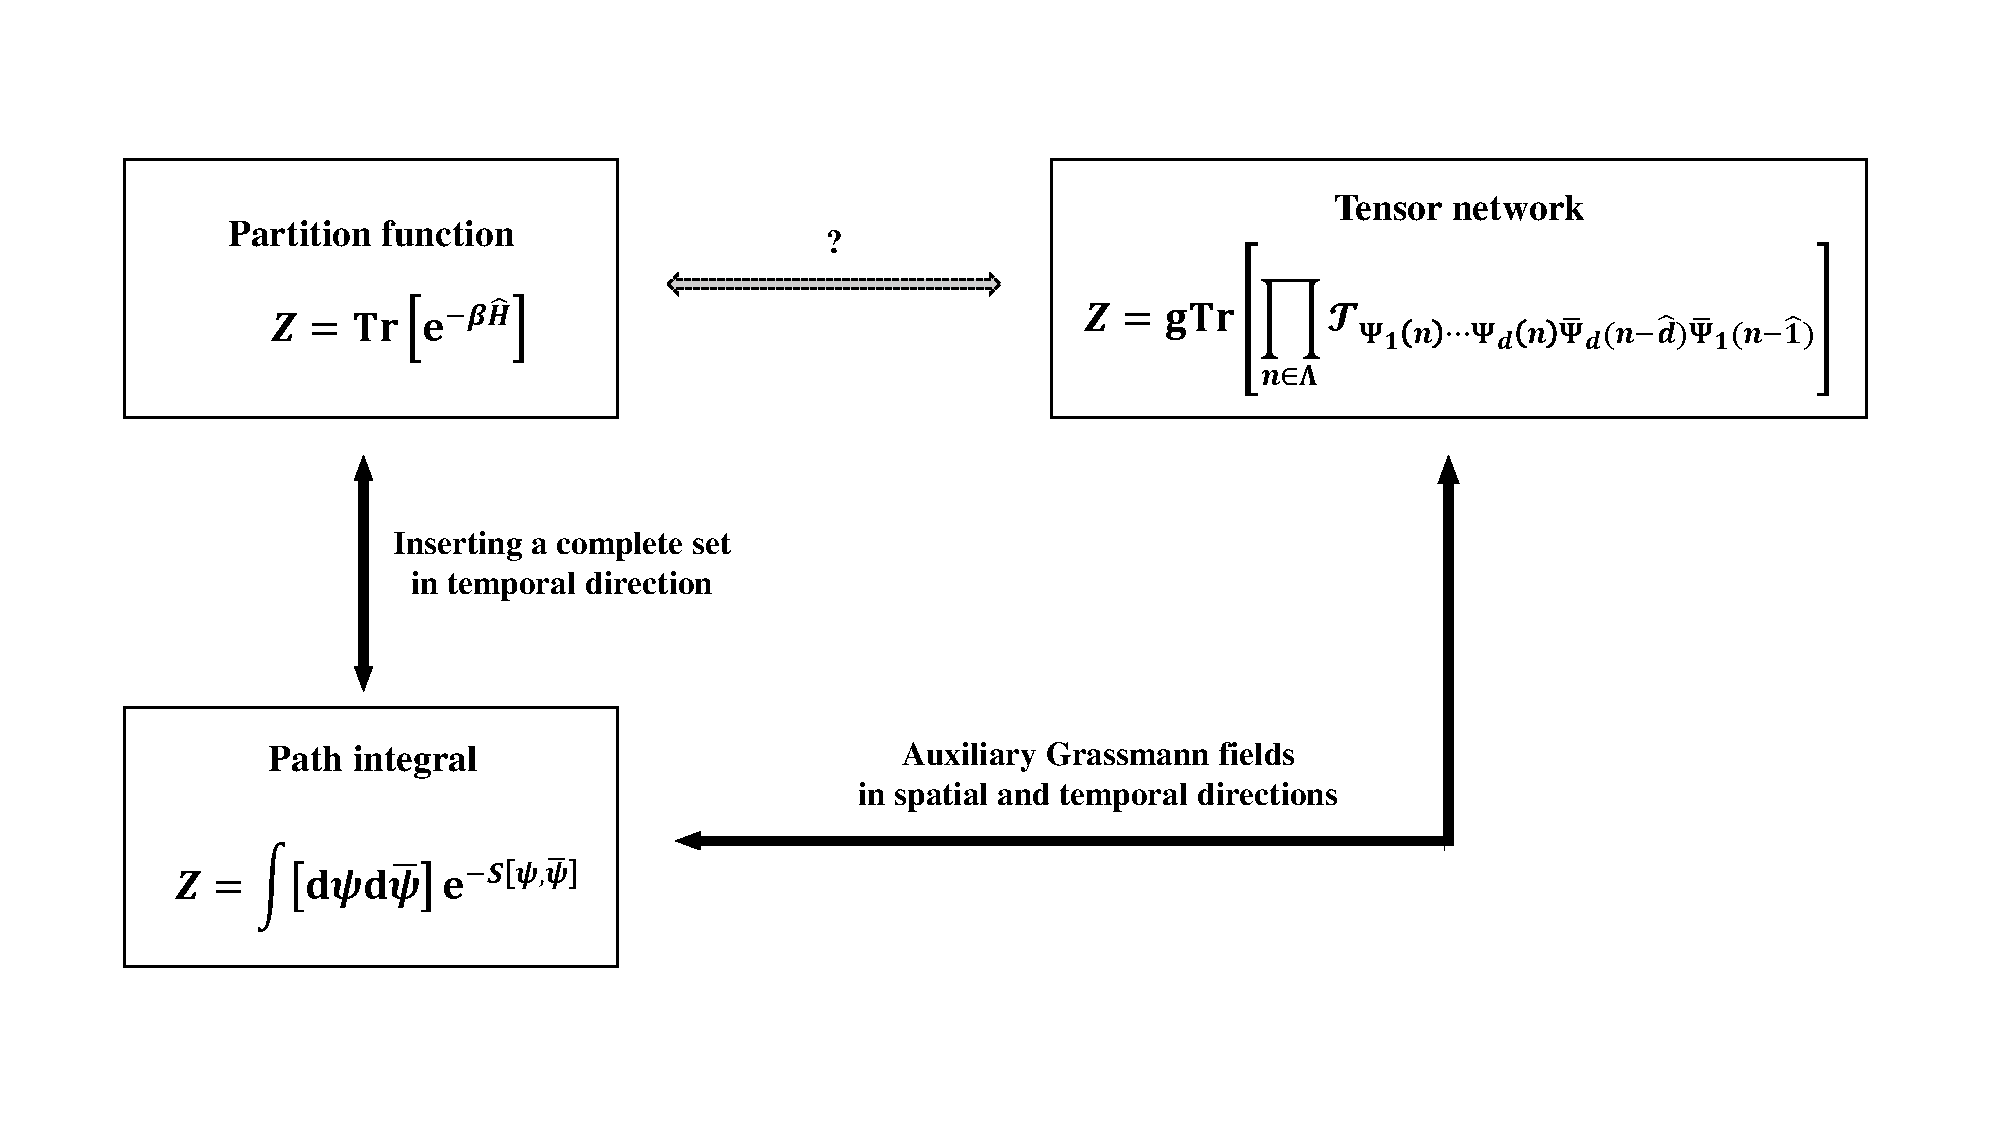
\includegraphics[width=1.1\hsize]{comm.pdf}
	\caption{A possible relationship between the path integral, partition function and tensor network.}
	\label{fig:commutative}
\end{figure}


%We have seen that, as with spin models, the current tensor network formulation for lattice fermions enables us to implement the coarse-graining algorithms based on direct truncation of degrees of freedom. It is known that some of these algorithms can be improved by removing the short-range correlation \cite{PhysRevLett.115.180405,PhysRevB.95.045117,PhysRevLett.118.110504,Hauru:2017tne,PhysRevB.97.045124}. The appliability of these types of algorithms to lattice fermion theories will be investigated as a future work.
